%           - Header-           %
\documentclass[a4paper, 11pt, fleqn, notitlepage, egregdoesnotlikesansseriftitles]{scrartcl}
\usepackage[english, ngerman]{babel}                % Sprache: Deutsch
\usepackage[utf8]{inputenc}                         % Dateiformat
\usepackage[T1]{fontenc}                            % Schriftsatz

%       - wichtige Pakete -     %
\usepackage{kpfonts}                                % Schrift
\usepackage{geometry}                               % Struktur
\usepackage{hyperref}                               % klickbare links
\usepackage{amsmath, amssymb, mathtools}            % mathematische Formeln
\usepackage[headsepline]{scrlayer-scrpage}          % Kopf- und Fußzeilen konfigurieren

%       - nuetzliche Pakete -   %
%\usepackage{tabularx}                              % schöne tabellen
%\usepackage{booktabs}                              % Trennlinien in Tabellen
%\setlength{\columnsep}{0.7cm}                      % Spaltenabstand
%\usepackage{multicol}                              % mehrspaltiger Text
\usepackage{graphicx}                               % Grafiken
%\usepackage[section]{placeins}
%\usepackage{tikz}                                  % Grafiken und Graphen
%\usepackage{diagbox}                               % Tabellen unterteilen
%\usepackage{bussproofs}                            % Logik und Kalkuele
%\usepackage{nicefrac}                              % schraege Brüche

% BibLateX
%\usepackage[backend=biber, authordate, eprint=false, url=false, block=ragged, bibencoding=inputenc]{biblatex-chicago}
%\usepackage{csquotes}
%\bibliography{quellen}                             % Quellen

%       - Eigene Befehle -      %
\newcommand{\emptyline}{\vspace{\baselineskip}}     % erzeugt leerzeile

%\newcommand{\N}{\mathbb{N}}
%\newcommand{\Z}{\mathbb{Z}}
%\newcommand{\R}{\mathbb{R}}
%\newcommand{\C}{\mathbb{C}}
%\newcommand{\Pf}{\mathbb{P}}

\newcommand{\aufgabe}{Block 7}
\newcommand{\modul}{Rechnernetze und Verteilte Systeme}
\newcommand{\sem}{Wintersemester 18/19}
\newcommand{\autorA}{Daniel Wujecki}
\newcommand{\autorB}{Amro Hendawi}
\newcommand{\autorC}{Nils Hendrischke}
\newcommand{\autorD}{Leon Marius Moll}
\newcommand{\autoren}{Wujecki, Hendawi, Hendrischke, Moll}
\newcommand{\uni}{Technische Universität Berlin}
\newcommand{\datum}{\today}

%       - Einstellungen -       %
\title{\aufgabe}
\subtitle{\modul}
\author{\name}
\date{\datum}

%\setlength{\parindent}{0pt}                                        % einruecken verhindern
\pagestyle{scrheadings}
\setcounter{secnumdepth}{0}                                        % keine Nummerierung von Überschriften
\geometry{left=25mm,right=20mm, top=27mm, bottom=25mm}              % bestimmte Seitenraender

\ihead{\aufgabe}
\chead{}
\ohead{\autoren}

\begin{document}

%         - Ttielseite -        %
%\maketitle
\thispagestyle{scrplain}

\noindent\Large
\textbf{\aufgabe} \hfill \textbf{\modul} \\
\normalsize
\autorA \hfill \uni \\
\autorB \hfill \sem \\
\autorC \hfill \datum \\
\autorD \hfill T18 G01 \\
\rule{\textwidth}{0.1mm}

%     - Inhaltsverzeichnis -    %
%\tableofcontents
%\newpage

%            - Text -           %

\section{a) Wie viele Pakete umfasst der Trace?}
Der Trace umfasst 15892 Pakete.

\section{b) Wie groß sind die Pakete im Durchschnitt?}
Sie sind im Durchschnitt 897,98 groß.

\section{c) Notieren Sie alle im Trace auftauchenden MAC-Adressen.}

\begin{itemize}
    \item 00:0c:29:b6:b5:48
    \item 00:50:56:f3:f2:f6
    \item 33:33:00:01:00:03
    \item 01:00:5e:00:00:fc
    \item 00:50:56:c0:00:08
\end{itemize}

\section{d) Wie viele IP-Adressen tauchen im Trace auf?}

\begin{itemize}
    \item \textbf{IPv4:} 53
    \item \textbf{IPv6:} 2
\end{itemize}

\section{e) Einige der auftauchenden MAC-Adressen sind mit IP-Adressen verknupft. Notieren sie diese Verknüpfungen.}

Folgende Mac Adressen sind mit Ip Adressen verknüpft:
\begin{itemize}
    \item 00:0c:29:b6:b5:48 mit 172.16.254.128
    \item 00:50:56:f3:f2:f6 mit 172.16.254.2
\end{itemize}

\section{f) Bei welchem Anteil der Pakete wird das Internet Protocol (IP) auf der Vermittlungs/Netzwerkschicht (ISO/OSI Modell) verwendet?}
Bei 100 Prozent.

\section{g) Bei welchem Anteil der Pakete wird das Transmission Control Protocol (TCP) auf der Transportschicht verwendet?}
Bei 98,2 Prozent.

\section{h) Notieren Sie alle Protokolle der Applikationsschicht die TCP nutzen.}
\begin{itemize}
    \item HTTP
\end{itemize}

\section{i) Notieren Sie alle Protokolle der Applikationsschicht die das User Datagram Protocol (UDP) nutzen.}
\begin{itemize}
    \item NetBIOS Name Service
    \item Link-local Multicast Name Resolution
    \item Dropbox LAN sync Discovery Protocol
    \item Domain Name System
\end{itemize}

\section{j) Notieren sie alle auftauchenden Protokolle der Vermittlungs/Netzwerkschicht.}
\begin{itemize}
    \item IPv4
    \item IPv6
\end{itemize}

\section{k) Notieren sie alle auftauchenden Protokolle der Sicherungsschicht.}
ARP

\section{l) Wie viele Domain Name System (DNS)-Abfragen fanden statt?}
Es fanden 195 DNS-Abfragen statt.

\section{m) Wie viele IP-Pakete haben einen “Time-To-Live” (TTL) Wert großer als 200, mit genau 128 und mit genau 64? Versuchen sie, eine Erklarung für die gefundene Verteilung zu finden.}

Es gab:
\begin{itemize}
    \item 0 Pakete mit einer TTL > 200
    \item 15833 Pakete mit einer TTL = 128
    \item 6 Pakete mit einer TTL = 64
\end{itemize}

64 und 128 sind Standardwerte, die sich jedoch bei verschiedenen Systemen unterscheiden.

\pagebreak
\section{n) Untersuchen Sie das 16. Paket im Trace genauer:}

\subsection{1. Wie groß ist der Ethernet-Header?}

Er ist 14 groß.

\subsection{2. Wie groß ist der IP-Header?}

Er ist 20 Bytes groß.

\subsection{3. Wie groß ist das IP-Datagram?}

Er ist 193 Bytes groß.

\subsection{4. Wie groß ist der TCP-Header?}

Er ist 20 Bytes groß.

\subsection{5. Wie groß ist das TCP-Segment?}

Er ist 153 Bytes groß.

\section{o)Erstellen Sie ein Histogramm über die Länge der IP-Datagramme. Interpretieren Sie das Ergebnis.}

\begin{center}
    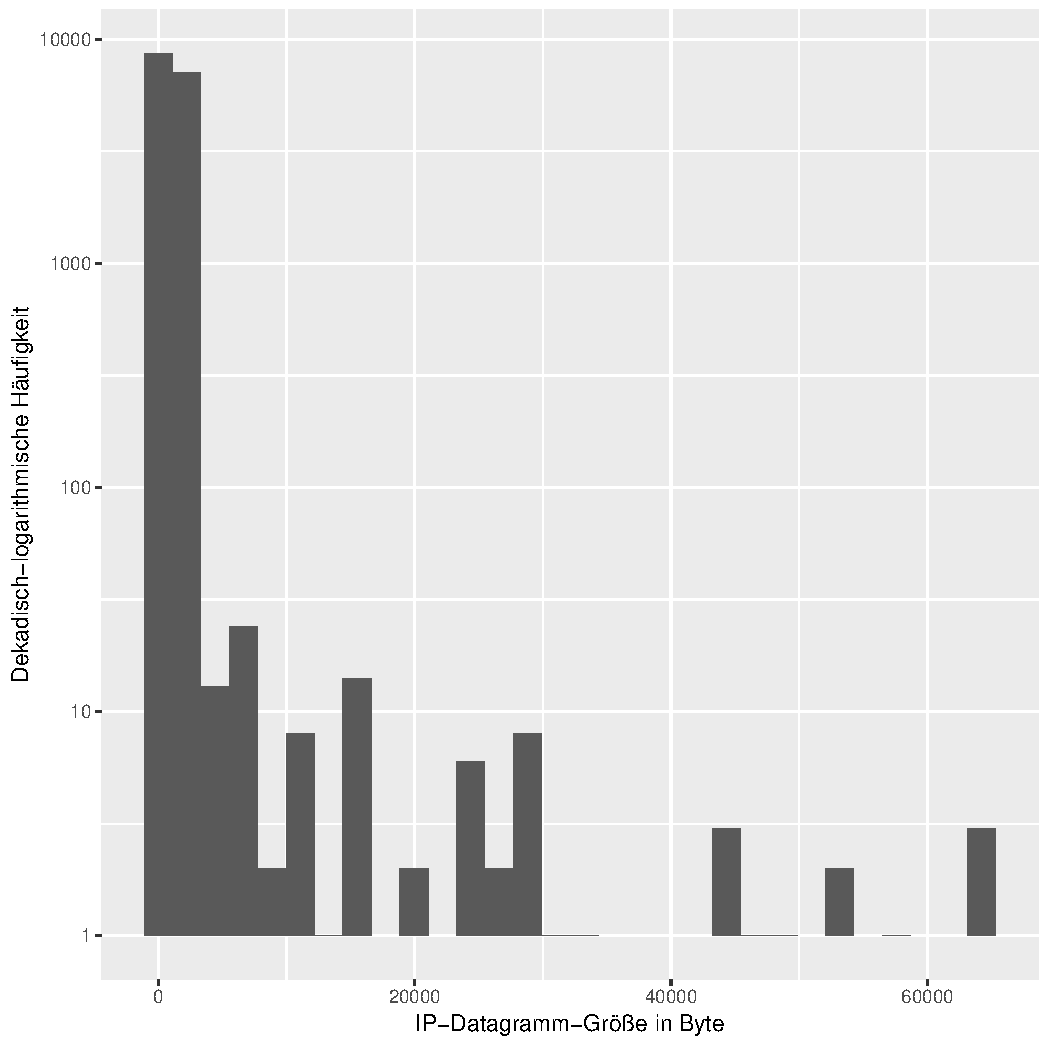
\includegraphics[width=\textwidth]{length_all}
    \captionof{figure}{Histogram: Länge aller IP-Datagramme}
    \label{fig:hist:all}
\end{center}
Ein Großteil der IP-Datramm Pakete ist sehr kurz. Dies ist wie folgt zu erklären: Wenn man die Kommunikation in viele kleine Pakete unterteilt, ist der Schaden eines einzelnen Paketverlusts geringer als bei wenigen großen Paketen. Da zu über 98 \% TCP verwendet wurde und dort die Chance des Paketverlusts erheblich höher als bei UDP ist, sind die Pakete zum Großteil kurz.

\section{p)Zwischen welchen IP-Adressen werden die meisten Bytes ausgetauscht? Erstellen Sie ein Histogramm über die Länge dieser IP-Datagramme. Interpretieren Sie das Ergebnis.}

Die Grund der Verteilung ist der gleiche wie bei Aufgabe o) und dieser bitte zu entnehmen.
Zwischen 81.166.122.238 und 172.16.254.128 wurden am meisten Bytes ausgetauscht.

\begin{center}
    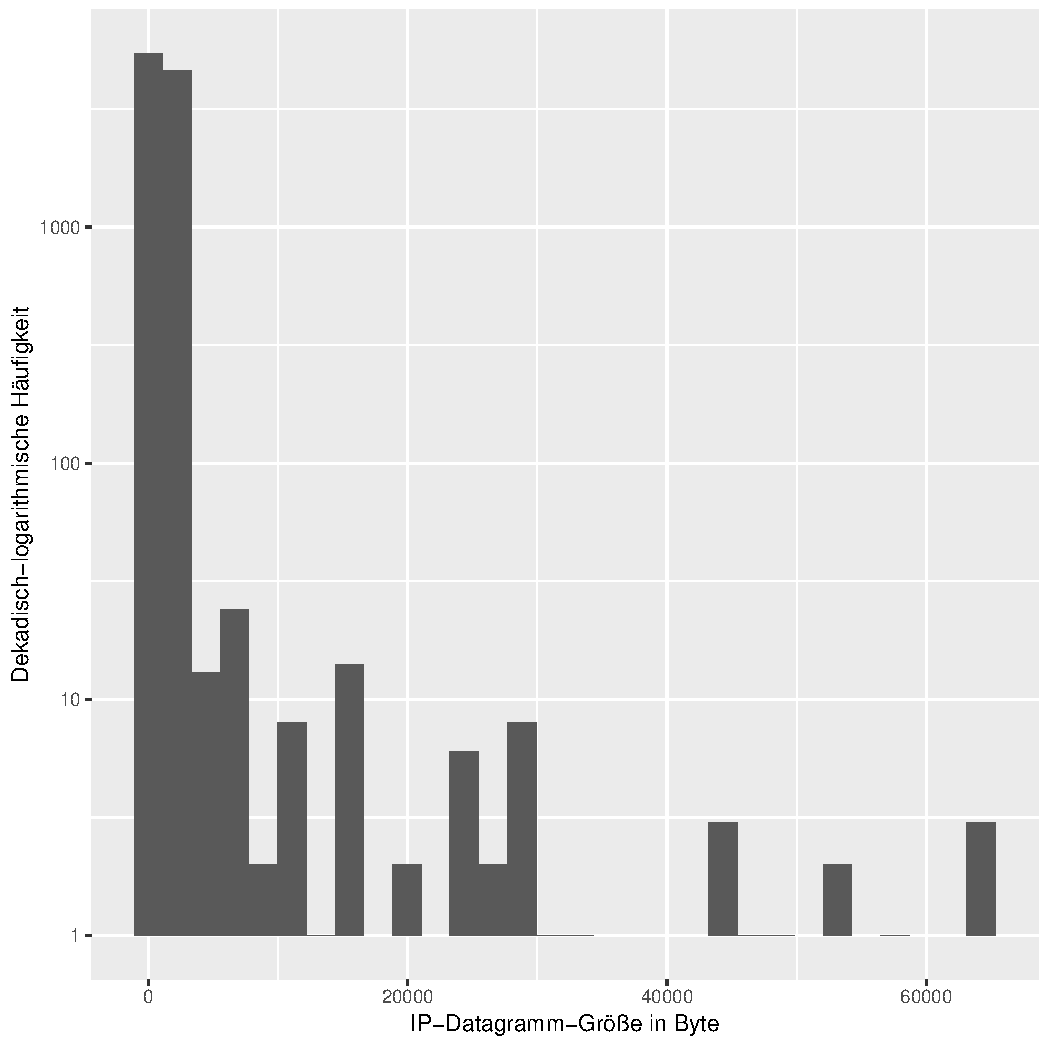
\includegraphics[width=\textwidth]{length_ausschnitt}
    \captionof{figure}{Histogram: Länge einiger IP-Datagramme}
    \label{fig:hist:some}
\end{center}

\section{q) Zwischen welchen IP-Adressen werden die meisten Pakete ausgetauscht?}
Zwischen 81.166.122.238 und 172.16.254.128 wurden am meisten Pakete ausgetauscht.

\section{r) Bestand eine verschlüsselte Verbindung? Notieren Sie ggf. die beteiligten Hosts}

Bei 1368 Paketen bestand eine verschlüsselte Verbindung.
Folgende Hosts mit folgenden IP-Adressen waren beteiligt:
\begin{itemize}
    \item 23.192.162.171
    \item 23.205.82.104
    \item 31.13.93.3
    \item 54.227.250.135
    \item 88.221.83.67
    \item 88.221.83.80
    \item 172.16.254.128
\end{itemize}

\section{s) Wurde ein Web-Browser benutzt? Wenn ja, welche?}
Es wurde Chrome in der Version 41 und 40 benutzt.

%     - Quellenverzeichnis -    %
%\newpage
%\printbibliography

\end{document}
